\section{仮想化技術と仮想マシン}
\tocc
\newcommand{\ie}{\tikz{\draw[arrows={-Latex[line width=1pt,fill=white,length=10pt]}](0,0)--(1,0)}\ }
\begin{frame}[t]{\thesection.\ \secname}
    \newcommand{\server}{サーバー}
    \begin{block}{仮想化}
        ``コンピューターの物理的資源を論理的に分割して,それぞれ独立並列した状態で利用できるようにすること.
        1台の\server で,複数の基本ソフトを独立並列に動作させる\server 仮想化など.''\hfill\cite{スーパー大辞林}
    \end{block}
    \ie 1台の計算機で複数のOSやアプリケーションなどを並列に動作させること.
    \vspace{.5em}
    \begin{block}{Virtual Machine(仮想機械,仮想マシン)}
        ``あるコンピューターシステムの動作を,別システムで再現するソフトウエア.また,そのような動作環境.あるOSの動作を別のOS上で再現する場合など.バーチャルマシン.VM.''\hfill\cite{スーパー大辞林}
    \end{block}
    \ie 仮想化するためのソフトウェアや動作環境.
\end{frame}
\begin{frame}{\thesection.\ \secname}
    \begin{figure}
        \centering
        \begin{minipage}[b]{.48\textwidth}
            \centering
            \begin{tikzpicture}
                \node[str,fill=gray!60,text width=.42\textwidth](hw1){物理サーバ};
                \node[str,fill=gray!40,text width=.42\textwidth,above=.1cm of hw1](os1){OS};
                \node[str,fill=gray!20,text width=.42\textwidth,above=.1cm of os1](sw1){\scriptsize アプリケーション};
                \node[str,fill=gray!60,text width=.42\textwidth,right=.1cm of hw1](hw2){物理サーバ};
                \node[str,fill=gray!40,text width=.42\textwidth,above=.1cm of hw2](os2){OS};
                \node[str,fill=gray!20,text width=.42\textwidth,above=.1cm of os2](sw2){\scriptsize アプリケーション};
                \node[inner sep=.05cm,draw,rounded corners,fit={(hw1)(os1)(sw1)}](warp1){};
                \node[inner sep=.05cm,draw,rounded corners,fit={(hw2)(os2)(sw2)}](warp2){};
            \end{tikzpicture}
            仮想化前
        \end{minipage}
        \begin{minipage}[b]{.48\textwidth}
            \centering
            \begin{tikzpicture}
                \node[str,fill=gray!60,text width=.85\textwidth](hw1){ハードウェア};
                \node[str,fill=gray!50,text width=.85\textwidth,above=.1cm of hw1](vmm){仮想化ソフトウェア};
                \node[str,fill=gray!40,text width=.38\textwidth,above=.1cm of vmm.north east,anchor=south east](os1){OS};
                \node[str,fill=gray!40,text width=.38\textwidth,above=.1cm of vmm.north west,anchor=south west](os2){OS};
                \node[str,fill=gray!20,text width=.38\textwidth,above=.1cm of os1](sw1){\tiny アプリケーション};
                \node[str,fill=gray!20,text width=.38\textwidth,above=.1cm of os2](sw2){\tiny アプリケーション};
                \node[inner sep=.05cm,draw,rounded corners,fit={(hw1)(vmm)},draw=white](warp1){};

            \end{tikzpicture}
            仮想化後
        \end{minipage}
    \end{figure}
\end{frame}
\section{仮想化の方式}
\tocc
\subsection{ホスト型}
\begin{frame}[t]{\ftitle}
    ハードウェアの中のOS上に,土台となる仮想ソフトウェアをインストールし,仮想化ソフトウェアで仮想マシンを稼働させる.
    \begin{figure}[b]
        \centering
        \begin{tikzpicture}
            \node[str,fill=gray!60,text width=.9\textwidth](hw){ハードウェア};
            \node[str,fill=gray!50,text width=.9\textwidth,above=.1cm of hw](hos){ホストOS};
            \node[str,fill=gray!40,text width=.9\textwidth,above=.1cm of hos](hsw){ホスト型仮想化ソフトウェア};
            \node[str,fill=gray!30,text width=.43\textwidth,above=.1cm of hsw.north west,anchor=south west](gos1){ゲストOS};
            \node[str,fill=gray!30,text width=.43\textwidth,above=.1cm of hsw.north east,anchor=south east](gos2){ゲストOS};
            \node[str,fill=gray!20,text width=.2\textwidth,above=.1cm of gos1.north west,anchor=south west](sw1){\tiny アプリケーション};
            \node[str,fill=gray!20,text width=.2\textwidth,above=.1cm of gos1.north east,anchor=south east](sw2){\tiny アプリケーション};
            \node[str,fill=gray!20,text width=.2\textwidth,above=.1cm of gos2.north west,anchor=south west](sw3){\tiny アプリケーション};
            \node[str,fill=gray!20,text width=.2\textwidth,above=.1cm of gos2.north east,anchor=south east](sw4){\tiny アプリケーション};
        \end{tikzpicture}
    \end{figure}
    % \hyperlink{ハイパーバイザ型}{\beamergotobutton{ハイパーバイザ型}}\hypertarget{ホスト型}{}
\end{frame}
\begin{frame}[t]{\ftitle}
    \begin{exampleblock}{ホスト型仮想化ソフトウェア 例}
        \begin{minipage}[b]{.8\textwidth}
            \begin{itemize}
                \setlength{\itemsep}{1em}
                \item VMware Workstation Player
                \item VMware Fusion
                \item Oracle VM Virtualbox
            \end{itemize}
        \end{minipage}
        \begin{minipage}[b]{.15\textwidth}
            \centering
            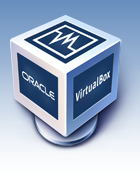
\includegraphics[keepaspectratio,width=.8\textwidth]{virtualbox_logo.png}\\
            {\tiny Virtualbox\cite{VMBox}}
        \end{minipage}
    \end{exampleblock}
    \begin{minipage}[t]{.48\textwidth}
        \textbf{\cmark メリット}
        \begin{itemize}
            \item 既存マシンが利用できる点.
            \item 仮想化に必要なソフトウェアが扱いやすい.
        \end{itemize}
    \end{minipage}
    \begin{minipage}[t]{.48\textwidth}
        \textbf{\xmark デメリット}
        \begin{itemize}
            \item ホストOSを動作させるための物理リソースが必要.
        \end{itemize}
    \end{minipage}\\
    \hfill\cite{itmanage}
\end{frame}
\subsection{ハイパーバイザ型}
\begin{frame}[t]{\ftitle}
    ハイパーバイザとは「仮想化のためのOS」のようなもの.ホストOSを必要としない,仮想化ソフトウェア.
    \begin{figure}[b]
        \centering
        \begin{tikzpicture}
            \node[str,fill=gray!60,text width=.9\textwidth](hw){ハードウェア};
            \node[str,fill=gray!45,text width=.9\textwidth,above=.1cm of hw,minimum height=2.1cm](hpv){ハイパーバイザ};
            \node[str,fill=gray!30,text width=.43\textwidth,above=.1cm of hpv.north west,anchor=south west](gos1){ゲストOS};
            \node[str,fill=gray!30,text width=.43\textwidth,above=.1cm of hpv.north east,anchor=south east](gos2){Linux};
            \node[str,fill=gray!20,text width=.2\textwidth,above=.1cm of gos1.north west,anchor=south west](sw1){\tiny アプリケーション};
            \node[str,fill=gray!20,text width=.2\textwidth,above=.1cm of gos1.north east,anchor=south east](sw2){\tiny アプリケーション};
            \node[str,fill=gray!20,text width=.2\textwidth,above=.1cm of gos2.north west,anchor=south west](sw3){Apache};
            \node[str,fill=gray!20,text width=.2\textwidth,above=.1cm of gos2.north east,anchor=south east](sw4){Python};
        \end{tikzpicture}
    \end{figure}
    % \hyperlink{ホスト型}{\beamergotobutton{ホスト型}}\hypertarget{ハイパーバイザ型}{}
\end{frame}
\begin{frame}[t]{\ftitle}
    \begin{exampleblock}{ハイパーバイザ 例}
        \begin{itemize}
            \item VMware ESXi
            \item Linux KVM
            \item Microsoft Hyper-V
        \end{itemize}
    \end{exampleblock}
    \begin{minipage}[t]{.48\textwidth}
        \textbf{\cmark メリット}
        \begin{itemize}
            \item ホスト型に比べて,システム全体の観点から見てリソースの使用効率がよい.
            \item 物理サーバに比べて,運用にかかるコストを削減できる.
        \end{itemize}
    \end{minipage}
    \begin{minipage}[t]{.48\textwidth}
        \textbf{\xmark デメリット}
        \begin{itemize}
            \item 物理サーバに比べて,性能が劣る.
            \item 物理サーバに比べて,障害の範囲は大きくなる(ことがある.)
        \end{itemize}
    \end{minipage}\\
    \hfill\cite{itmanage}
\end{frame}
\subsection{コンテナ型}
\begin{frame}[t]{\ftitle}
    ``アプリケーションを実行するための領域(ユーザ空間)を複数に分割して利用するもの''\cite{itmanage}.
    \begin{figure}[b]
        \centering
        \begin{tikzpicture}
            \node[str,fill=gray!60,text width=.9\textwidth](hw){ハードウェア};
            \node[str,fill=gray!50,text width=.9\textwidth,above=.1cm of hw](hos){ホストOS};
            \node[str,fill=gray!40,text width=.9\textwidth,above=.1cm of hos](hsw){Docker または Kubernetes};
            \node[str,fill=gray!30,text width=.2\textwidth,above=.1cm of hsw.north west,anchor=south west](gos1){ミドルウェア};
            \node[str,fill=gray!30,text width=.2\textwidth,above=.1cm of hsw.north east,anchor=south east](gos2){DBMS};
            \node[str,fill=gray!20,text width=.2\textwidth,above=.1cm of gos1.north west,anchor=south west](sw1){\tiny アプリケーション};
            \node[str,fill=gray!20,text width=.2\textwidth,above=.1cm of gos2.north east,anchor=south east](sw4){MySQL};
            \node[inner sep=.5mm,fit={(gos1)(sw1)},draw,thick,dotted,rounded corners](wrap1){};
            \node[inner sep=.5mm,fit={(gos2)(sw4)},draw,thick,dotted,rounded corners](wrap2){};
            \node at ($(wrap1)!0.5!(wrap2)+(0,.5cm)$)(cont){コンテナ};
            \draw[-latex](cont.west)--(wrap1.east);
            \draw[-latex](cont.east)--(wrap2.west);
        \end{tikzpicture}
    \end{figure}
\end{frame}
\begin{frame}[t]{\ftitle}
    \begin{block}{ミドルウェア}
        システムソフトウェアは,基本ソフトウェア(OS)とミドルウェアに分類される.
        ミドルウェアはOSとアプリケーションソフトウェアの中立ちをする.\hfill\cite{ITの基礎}
    \end{block}
    \begin{exampleblock}{ミドルウェアの例}
        データベースを管理する,データベースを操作する基本ソフトウェア(DBMS\footnote{Data Base Management System})がある.
    \end{exampleblock}
\end{frame}
\begin{frame}[t]{\ftitle}
    \begin{minipage}[t]{.48\textwidth}
        \textbf{\cmark メリット}
        \begin{itemize}
            \item バージョン依存が激しいもの(Python,JavaScript)などでも指定した環境を再現しやすい.(\texttt{Dockerfile})
            \item 環境構築が簡単.
            \item ゲストOSが不要なので,アプリケーションの起動や処理が高速.
        \end{itemize}
    \end{minipage}
    \begin{minipage}[t]{.48\textwidth}
        \textbf{\xmark デメリット}
        \begin{itemize}
            \item 同一基盤上で異なるOSを動かせない.
            \item ホストOSで障害が生じると,すべてのコンテナに影響が出る.
        \end{itemize}
    \end{minipage}
\end{frame}